\section{Comparing intervals with different confidence levels}
%%%%%%%%%%%%%%%%%%%%%%%%%%%%%%%%%%%%%%%%
%1\begin{frame}
%1\frametitle{How Much Narrower is a 68\% CI? \hfill \includegraphics[scale = 0.05]{./images/clicker}}
%1
%1Suppose we're constructing a confidence interval for the mean of a normal population with $\sigma^2$ known:
%1$$\bar{X}_n \pm \texttt{qnorm}(1 - \alpha /2) \times \sigma/\sqrt{n}$$
%1Approximately what is the \emph{ratio} of the width of a 95\% interval divided by that of a 68\% interval? 
%1
%1
%1\pause
%1
%1
%1\alert{$$
%1\boxed{\begin{array}{r}
%1	\texttt{qnorm}(1 - 0.05/2) \approx 2  \\
%1	\texttt{qnorm}(1 - 0.32/2)  \approx 1
%1\end{array}} \implies 
%1\frac{2 \times \texttt{qnorm}(1 - 0.05/2) \times \sigma/\sqrt{n}}{  2 \times \texttt{qnorm}(1 - 0.32/2) \times \sigma/\sqrt{n}}\approx 2
%1$$}
%1
%1\end{frame}
%1
%1%%%%%%%%%%%%%%%%%%%%%%%%%%%%%%%%%%%%%%%%


\begin{frame}

  \vspace{1em}

\begin{figure}
\centering
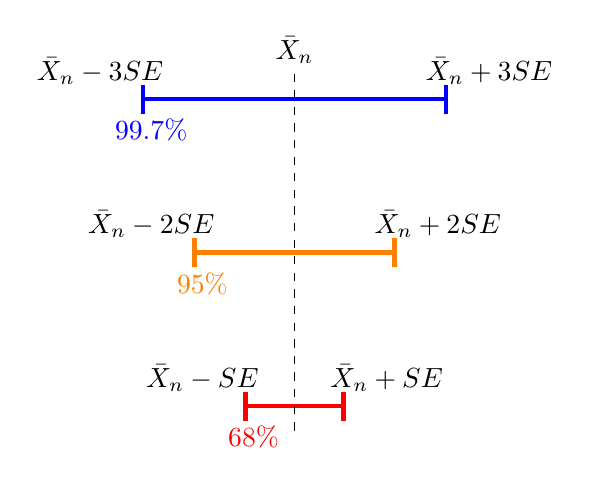
\begin{tikzpicture}[scale = 0.65]
	\draw [ultra thick, blue, |-|](-3,3) -- (3,3);
	\node [above] at (-3.8,3.1) {$\bar{X}_n-3 SE$};
	\node [above] at (3.8,3.1) {$\bar{X}_n+3  SE$};
	\node [below, blue] at (-2.8, 2.8) {99.7\%};	
	
	\draw [ultra thick, orange, |-|](-2,0) -- (2,0);
	\node [above] at (-2.8,0.1) {$\bar{X}_n-2 SE$};
	\node [above] at (2.8,0.1) {$\bar{X}_n+2 SE$};
	\node [below, orange] at (-1.8, -0.2) {95\%};	

	\draw [ultra thick, red, |-|](-1,-3) -- (1,-3);
	\node [above] at (-1.8,-2.9) {$\bar{X}_n -  SE$};
	\node [above] at (1.8,-2.9) {$\bar{X}_n +  SE$};
	\node [below, red] at (-0.8, -3.2) {68\%};	
	
	\draw [dashed](0,3.5) -- (0,-3.5);
	\node [above] at (0,3.5) {$\bar{X}_n$};	
\end{tikzpicture}
\singlespacing

\vspace{-1em}

\caption{\footnotesize  Each CI gives a range of ``plausible'' values for the population mean $\mu$, centered at the sample mean $\bar{X}_n$. Values near the middle are ``more plausible'' in the sense that a small reduction in confidence level gives a much shorter interval centered in the same place. This is because the sample mean is unlikely to take on values far from the population mean in repeated sampling.}
\end{figure}

\end{frame}
%%%%%%%%%%%%%%%%%%%%%%%%%%%%%%%%%%%%%%%%
\section{What if the population is normal but $\sigma$ is unknown?}
%%%%%%%%%%%%%%%%%%%%%%%%%%%%%%%%%%%%%%%%
\begin{frame}
  \frametitle{Assume that: $X_1, \dots, X_n \sim \text{iid N}(\mu, \sigma^2)$}

\begin{block}{$\sigma$ Known}
  \[P\left[ -\texttt{qnorm}(1 - \alpha/2) \leq \frac{\bar{X}_n - \mu}{\sigma/\sqrt{n}}\leq \texttt{qnorm}(1 - \alpha/2) \right] = 1 - \alpha\]

  \vspace{1em}
  $\implies$ Confidence Interval: $\alert{\bar{X}_n \pm \texttt{qnorm}(1 - \alpha/2) \times \sigma/ \sqrt{n}}$
\end{block}

\pause

\begin{block}{$\sigma$ Unknown}
  Idea: estimate $\sigma$ with $S$. Unfortunately: 

  \[
    \alert{\frac{\bar{X}_n - \mu}{S/\sqrt{n}} \quad \text{ IS NOT A NORMAL RV! }}
  \]

\end{block}

\end{frame}
%%%%%%%%%%%%%%%%%%%%%%%%%%%%%%%%%%%%%%%%
\begin{frame}
  \frametitle{50000 Simulation replications: $X_1, \dots, X_5 \sim \text{iid N}(\mu, \sigma^2)$}

  \vspace{3em}

  \begin{figure}
    \centering
\includegraphics[scale = 0.45, trim = 2cm 2cm 2cm 2cm]{./images/normal_vs_t_sampling}
\caption{In each plot the red curve is the pdf of the standard normal RV. At left: the sampling distribution of $\sqrt{5}(\bar{X}_5 - \mu)/\sigma$ is standard normal. At right: the sampling distribution of $\sqrt{5}(\bar{X}_5 - \mu)/S$ clearly isn't!}
\end{figure}

\end{frame}
%%%%%%%%%%%%%%%%%%%%%%%%%%%%%%%%%%%%%%%%

\begin{frame}
  \frametitle{Student-t Random Variable}
If $X_1, \hdots, X_n \sim \mbox{iid } N(\mu,\sigma^2)$, then
	$$\alert{\boxed{\frac{\bar{X}_n - \mu}{S/\sqrt{n}} \sim t(n-1)}}$$


\begin{itemize}
  \item Parameter: $\nu = n-1$ ``degrees of freedom'' 
	\item Support = $(-\infty, \infty)$
	\item Symmetric around zero, but mean and variance may not exist!
	\item Degrees of freedom $\nu$ control ``thickness of tails''
	\item As $\nu \rightarrow \infty$, $t \rightarrow$ Standard Normal.
\end{itemize}
\vspace{1em}


\end{frame}

%%%%%%%%%%%%%%%%%%%%%%%%%%%%%%%%%%%%%%%%
\begin{frame}
\frametitle{Student-t PDFs}

\begin{figure}
\includegraphics[scale = 0.58]{./images/tpdf}
\end{figure}
\end{frame}

%%%%%%%%%%%%%%%%%%%%%%%%%%%%%%%%%%%%%%%%
\begin{frame}
\frametitle{Who was ``Student?''}
\framesubtitle{\href{http://www.aeaweb.org/articles.php?doi=10.1257/jep.22.4.199}{\fbox{``Guinnessometrics: The Economic Foundation of Student's t''}}}

\begin{columns}

\column{0.3\textwidth}
\begin{figure}
\fbox{\includegraphics[scale = 0.045]{./images/gosset}}
\vspace{0.75em}

\includegraphics[scale = 0.15]{./images/guinness}
\end{figure}


\column{0.7\textwidth}
\scriptsize
\begin{quote}
``Student'' is the pseudonym used in 19 of 21 published articles by William Sealy
Gosset, who was a chemist, brewer, inventor, and self-trained statistician, agronomer, and designer of experiments ... [Gosset] worked his entire adult life ... as an experimental brewer for one employer: Arthur Guinness, Son \& Company, Ltd., Dublin, St.\ James’s Gate. Gosset was a master brewer and rose in fact to the top of the top of the brewing industry: Head Brewer of Guinness.
\end{quote}

\end{columns}

\end{frame}

%%%%%%%%%%%%%%%%%%%%%%%%%%%%%%%%%%%%%%%%

\begin{frame}
\frametitle{CI for Mean of Normal Distribution, Popn.\ Var.\ Unknown}
Same argument as we used when the variance was known, except with $t(n-1)$ rather than standard normal distribution:
	\begin{eqnarray*}
		P\left(-c \leq \frac{\bar{X}_n-\mu}{S/\sqrt{n}} \leq c \right) &=& 1-\alpha \\ \\ 
		P\left(\bar{X}_n - c \frac{S}{\sqrt{n}} \leq \mu\leq \bar{X}_n +c \frac{S}{\sqrt{n}} \right) &=& 1-\alpha 
	\end{eqnarray*}

\alert{$c =$ \texttt{qt}$(1-\alpha/2, \texttt{df} = n-1)$} 
	$$\boxed{\bar{X}_n \pm \texttt{qt}(1-\alpha/2, \texttt{df} = n-1)\;  \frac{S}{\sqrt{n}}}$$
\end{frame}



%%%%%%%%%%%%%%%%%%%%%%%%%%%%%%%%%%%%%%%%
\begin{frame}
\frametitle{Comparison of CIs for Mean of Normal Distribution}
\framesubtitle{$100\times(1-\alpha)\%$ Confidence Level}
$$\boxed{X_1, \hdots, X_n \sim \mbox{iid } N(\mu, \sigma^2)}$$


\begin{block}{Known Population Std.\ Dev.\ ($\sigma$)}
	$$\bar{X}_n \pm \; \texttt{qnorm}(1-\alpha/2) \; \frac{\sigma}{\sqrt{n}}$$
\end{block}


\begin{block}{Unknown Population Std.\ Dev.\ ($\sigma$)}
$$\bar{X}_n \pm \; \texttt{qt}(1-\alpha/2, \texttt{df} = n-1) \; \frac{S}{\sqrt{n}}$$
\end{block}
\end{frame}
%%%%%%%%%%%%%%%%%%%%%%%%%%%%%%%%%%%%%%%%%
\begin{frame}
\frametitle{Comparison of Normal and $t$ CIs}
\begin{table}
\caption{Values of \texttt{qt}$(1-\alpha/2, \texttt{df}=n-1)$ for various choices of $n$ and $\alpha$. }
\begin{tabular}{r|rrrrr|r}
\hline
$n$& 1& 5& 10& 30& 100 & $\infty$\\
\hline
$\alpha = 0.10$&  6.31& 2.02 & 1.81 & 1.70  & 1.66 &1.64\\
$\alpha = 0.05$ & 12.71& 2.57 & 2.23 & 2.04  & 1.98 &1.96\\
$\alpha = 0.01$ & 63.66& 4.03 & 3.17 & 2.75  & 2.63 &2.58\\
\hline
\end{tabular}
\end{table}
\alert{As $n\rightarrow \infty$, $t(n-1) \rightarrow N(0,1)$}
\vspace{1em}


In a sense, using the $t$-distribution involves making a ``small-sample correction.'' In other words, it is only when $n$ is fairly small that this makes a practical difference for our confidence intervals.
\end{frame}
%%%%%%%%%%%%%%%%%%%%%%%%%%%%%%%%%%%%%%%%

\begin{frame}
\frametitle{Am I Taller Than The Average American Male?}
\framesubtitle{\href{http://www.cdc.gov/nchs/data/series/sr_11/sr11_252.pdf}{\fbox{Source: Centers for Disease Control (pg.\ 16)}}}


\begin{columns}
\column{0.4\textwidth}
\footnotesize
		\begin{tabular}{|lr|}
		\hline
			Sample Mean & 69 inches\\
			Sample Std.\ Dev.\ & 6 inches\\
			Sample Size & 5647 \\
			\hline
			My Height & 73 inches\\
			\hline
		\end{tabular}

\begin{eqnarray*}
\widehat{SE}(\bar{X}_n) &=& s/\sqrt{n}\\
	& =& 6/\sqrt{5647}\\ 
	&\approx& 0.08
\end{eqnarray*}


\column{0.6\textwidth}
Assuming the population is normal,\\
$\boxed{\bar{X}_n \pm \; \texttt{qt}(1-\alpha/2, \texttt{df} = n-1) \; \widehat{SE}(\bar{X}_n)}$
	

\vspace{1em}
\alert{What is the approximate value of \texttt{qt(1-0.05/2, df = 5646)}?} \pause


\vspace{1em}
For large $n$, $t(n-1) \approx N(0,1)$, so the answer is approximately 2
\pause

 \vspace{1em}
\alert{What is the ME for the 95\% CI?} 

\pause $ME \approx 0.16 \implies69 \pm 0.16$

\end{columns}
 


\end{frame}
%%%%%%%%%%%%%%%%%%%%%%%%%%%%%%%%%%%%%%%%
\section{What if the population isn't normal? -- The Central Limit Theorem}
%%%%%%%%%%%%%%%%%%%%%%%%%%%%%%%%%%%%%%%%
\begin{frame}
\frametitle{The Central Limit Theorem}
Suppose that $X_1, \hdots, X_n$ are a random sample from a some population that is \alert{not necessarily normal} and has an unknown mean $\mu$.
Then, provided that $n$ is \alert{\emph{sufficiently large}}, 
$$\frac{\bar{X}_n -\mu}{S/\sqrt{n}} \approx N(0,1)$$

We will use this fact to create \emph{approximate} CIs for population mean even if we know \emph{nothing} about the population.
\end{frame}
%%%%%%%%%%%%%%%%%%%%%%%%%%%%%%%%%%%%%%%%
\begin{frame}
\frametitle{Example: Uniform(0,1) Population, $n = 20$}
\begin{figure}
\centering
\includegraphics[scale = 0.4]{./images/uniform_pdf}
\includegraphics[scale = 0.4]{./images/xbar_uniform}
\end{figure}
\end{frame}
%%%%%%%%%%%%%%%%%%%%%%%%%%%%%%%%%%%%%%%%
\begin{frame}
\frametitle{Example: $\chi^2(5)$ Population, $n = 20$}
\begin{figure}
\centering
\includegraphics[scale = 0.4]{./images/chisq_pop}
\includegraphics[scale = 0.4]{./images/xbar_chisq}
\end{figure}
\end{frame}
%%%%%%%%%%%%%%%%%%%%%%%%%%%%%%%%%%%%%%%%
\begin{frame}
\frametitle{Example: Bernoulli$(0.3)$ Population, $n =20$}
\begin{figure}
\centering
\includegraphics[scale = 0.4]{./images/bernoulli}
\includegraphics[scale = 0.4]{./images/xbar_bernoulli}
\end{figure}
\end{frame}
%%%%%%%%%%%%%%%%%%%%%%%%%%%%%%%%%%%%%%%%

%\begin{frame}
%\frametitle{Who is the Chief Justice of the US Supreme Court?\hfill \includegraphics[scale = 0.05]{./images/clicker}}
%	\begin{enumerate}[(a)]
%	\item Harry Reid
%	\item John Roberts
%	\item William Rehnquist
%	\item Stephen Breyer
%\end{enumerate}
%
%% \vspace{1em}
%% \alert{58/65 $\approx 90\%$ of the students in the class got this right. }
%
%\end{frame}
%%%%%%%%%%%%%%%%%%%%%%%%%%%%%%%%%%%%%%%%
\begin{frame}
\frametitle{Are US Voters Really That Ignorant?}
\framesubtitle{\fbox{\href{http://www.people-press.org/files/2012/08/8-10-12-Knowledge-release.pdf}{Pew: ``What Voters Know About Campaign 2012''}}}

\begin{block}{The Data}
Of 771 registered voters polled, only 39\% correctly identified John Roberts as the current chief justice of the US Supreme Court.
\end{block}

\begin{block}{Research Question}
Is the majority of voters unaware that John Roberts is the current chief justice, or is this just sampling variation?
\end{block}

\alert{Assume Random Sampling...}

\end{frame}
%%%%%%%%%%%%%%%%%%%%%%%%%%%%%%%%%%%%%%%%
\section{CI for a Proportion Using the Central Limit Theorem}
%%%%%%%%%%%%%%%%%%%%%%%%%%%%%%%%%%%%%%%%
\begin{frame}
\frametitle{Confidence Interval for a Proportion}
	\begin{block}{What is the appropriate probability model for the sample?} 
$X_1, \hdots, X_n \sim \mbox{iid Bernoulli}(p)$, 1 = Know Roberts is Chief Justice
\end{block}


	\begin{block}{What is the parameter of interest?}
$p$ = Proportion of voters \emph{in the population} who know Roberts is Chief Justice.
\end{block}



\begin{block}{What is our estimator?} 
Sample Proportion: $\widehat{p} = (\sum_{i=1}^n X_i)/n$
\end{block}
\end{frame}
%%%%%%%%%%%%%%%%%%%%%%%%%%%%%%%%%%%%%%%%
\begin{frame}
\frametitle{Sample Proportion \emph{is} the Sample Mean!}
\small
$X_1, \hdots, X_n \sim \mbox{iid Bernoulli}(p)$
		$$\widehat{p} = \frac{1}{n} \sum_{i=1}^n X_i = \bar{X}_n$$

\pause


	\begin{eqnarray*}
		E[\widehat{p}] &=&  E\left(\frac{1}{n}\sum_{i=1}^n X_i\right) =  \frac{1}{n} \sum_{i=1}^n E[X_i] =   \frac{np}{n} =  p\\ \\ \pause
		Var(\widehat{p}) &=&  Var\left(\frac{1}{n}\sum_{i=1}^n X_i\right) = \frac{1}{n^2} \sum_{i=1}^n Var(X_i) = \frac{n p(1-p)}{n^2} =  \frac{p(1-p)}{n} \\ \\  \pause
		SE(\widehat{p}) &=&  \sqrt{Var(\widehat{p})} =  \sqrt{\frac{p(1-p)}{n}} \\ \\ \pause
		\widehat{SE}(\widehat{p}) &=&  \sqrt{\frac{\widehat{p}(1-\widehat{p})}{n}}
	\end{eqnarray*}

\end{frame}
%%%%%%%%%%%%%%%%%%%%%%%%%%%%%%%%%%%%%%%%
\begin{frame}
\frametitle{Central Limit Theorem Applied to Sample Proportion}

\begin{alertblock}{Central Limit Theorem: Intuition}
Sample means are approximately normally distributed provided the sample size is large even if the population is non-normal.
\end{alertblock}

\begin{columns}

\column{0.5\textwidth}
\begin{block}{CLT For Sample Mean}
  $$\frac{\bar{X}_n -\mu}{S / \sqrt{n}} \approx N(0,1)$$
\end{block}

\column{0.5\textwidth}
\begin{block}{CLT for Sample Proportion}
$$\frac{\widehat{p} -p}{\sqrt{\frac{\widehat{p}(1-\widehat{p})}{n}}} \approx N(0,1)$$
\end{block}
\end{columns}

\vspace{1em}
In this example, the population is Bernoulli$(p)$ rather than normal. The sample mean is $\widehat{p}$ and the population mean is $p$.

\end{frame}
%%%%%%%%%%%%%%%%%%%%%%%%%%%%%%%%%%%%%%%%
\begin{frame}
\frametitle{Approximate 95\% CI for Population Proportion}
$$\frac{\widehat{p} -p}{\sqrt{\frac{\widehat{p}(1-\widehat{p})}{n}}} \approx N(0,1)$$ 
	\begin{eqnarray*}
		P\left(-2 \leq\frac{\widehat{p} -p}{\sqrt{\frac{\widehat{p}(1-\widehat{p})}{n}}} \leq  2\right) &\approx& 0.95\\ \\ 
		P\left(\widehat{p} - 2 \sqrt{\frac{\widehat{p}(1-\widehat{p})}{n}} \leq p \leq \widehat{p} + 2\sqrt{\frac{\widehat{p}(1-\widehat{p})}{n}}\right) &\approx& 0.95
	\end{eqnarray*}
\end{frame}



%%%%%%%%%%%%%%%%%%%%%%%%%%%%%%%%%%%%%%%%
\begin{frame}
\frametitle{$100\times(1-\alpha)$ CI for Population Proportion $(p)$}
$X_1, \hdots, X_n \sim \mbox{iid Bernoulli}(p)$
	$$\widehat{p} \pm \texttt{qnorm}(1-\alpha/2) \sqrt{\frac{\widehat{p}(1-\widehat{p})}{n}}$$
	\alert{Approximation based on the CLT. Works well provided $n$ is large and $p$ isn't too close to zero or one.}
\end{frame}
%%%%%%%%%%%%%%%%%%%%%%%%%%%%%%%%%%%%%%%%

\begin{frame}
\frametitle{Example: Bernoulli$(0.9)$ Population, $n =20$}
\begin{figure}
\centering
\includegraphics[scale = 0.4]{./images/bernoulli_bad}
\includegraphics[scale = 0.4]{./images/xbar_bernoulli_bad}
\end{figure}
\end{frame}
%%%%%%%%%%%%%%%%%%%%%%%%%%%%%%%%%%%%%%%%
\begin{frame}
\frametitle{Example: Bernoulli$(0.9)$ Population, $n =100$}
\begin{figure}
\centering
\includegraphics[scale = 0.4]{./images/bernoulli_bad}
\includegraphics[scale = 0.4]{./images/xbar_bernoulli_fixed}
\end{figure}
\end{frame}
%%%%%%%%%%%%%%%%%%%%%%%%%%%%%%%%%%%%%%%%
\begin{frame}
\frametitle{Approximate 95\% CI for Population Proportion\hfill \includegraphics[scale = 0.05]{./images/clicker}}
39\% of 771 Voters Polled Correctly Identified Chief Justice Roberts

\begin{eqnarray*}
	\widehat{SE}(\widehat{p}) &=& \sqrt{\frac{\widehat{p}(1-\widehat{p})}{n}} = \sqrt{\frac{(0.39)(0.61)}{771}}\\ 
	&\approx& 0.018 
\end{eqnarray*}

\alert{What is the ME for an approximate 95\% confidence interval?} \pause

$$ME \approx 2 \times \widehat{SE}(\bar{X}_n) \approx 0.04$$ \pause

\vspace{-1em}

What can we conclude?
\vspace{-1em}
$$\alert{\boxed{\mbox{Approximate 95\% CI: } \; (0.35, 0.43)}}$$

\end{frame}

%%%%%%%%%%%%%%%%%%%%%%%%%%%%%%%%%%%%%%%%

